\documentclass{standalone}
\usepackage[dvipsnames]{xcolor}
\usepackage{tikz}
\usetikzlibrary{calc, matrix, positioning, arrows.meta, decorations.pathreplacing}

\colorlet{Memory}{Melon!50}
\colorlet{Thread}{SkyBlue!50}
\colorlet{8bit}{LimeGreen}

\begin{document}

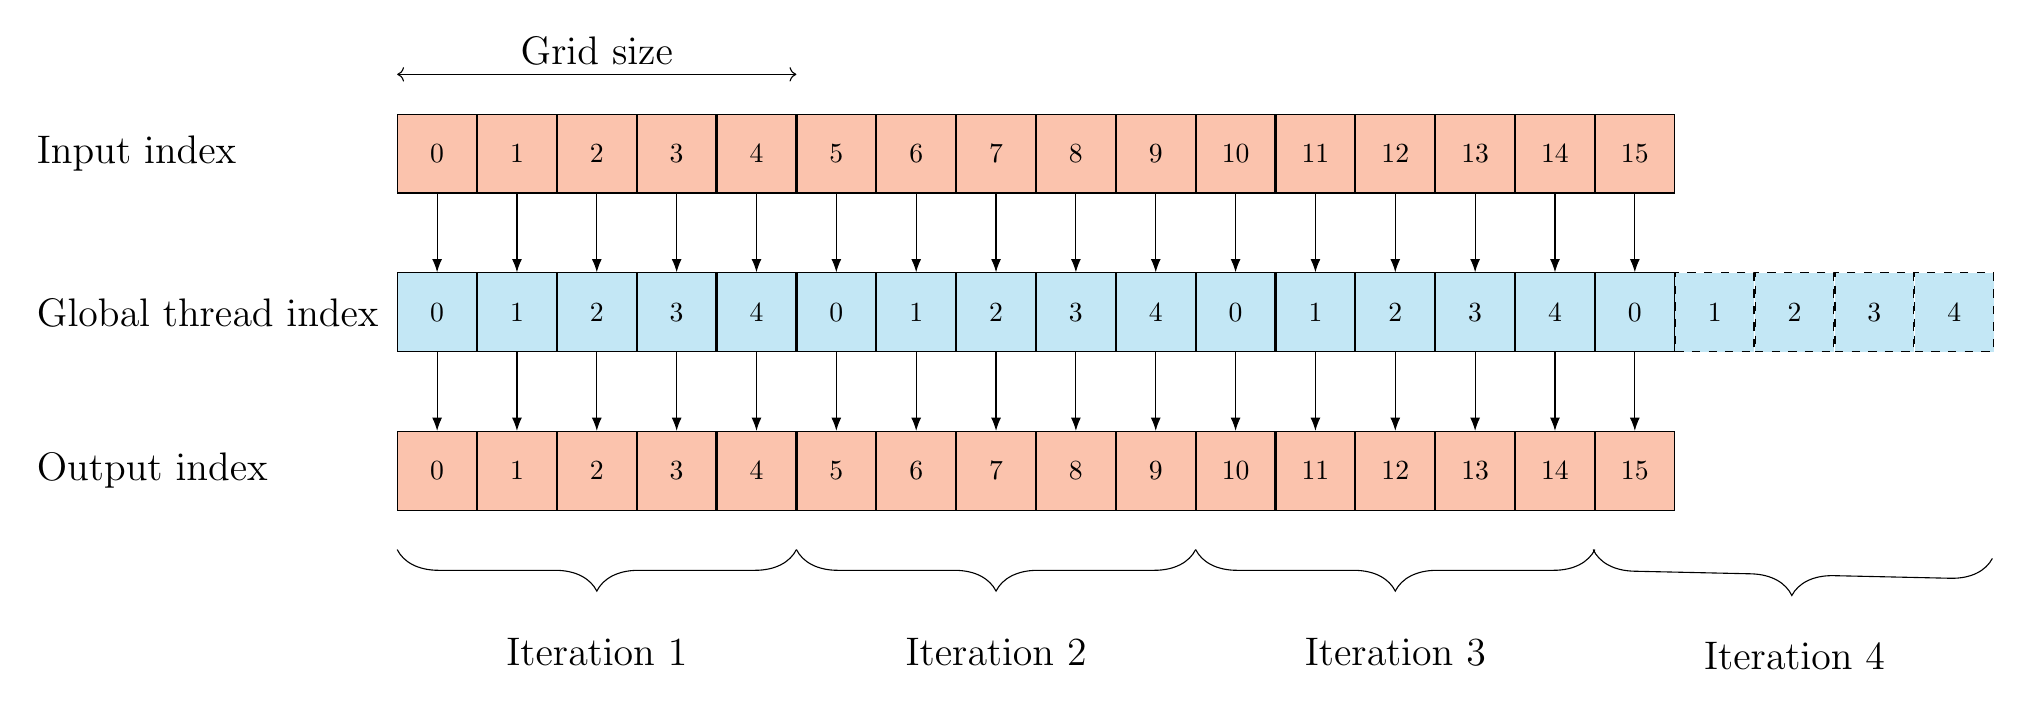
\begin{tikzpicture}[
  gpunode/.style={rectangle,draw=black,minimum width=1cm, minimum height=1cm},
  label/.style={font=\Large}
]

\matrix [
matrix of nodes,
nodes={gpunode},
row sep=1cm,
row 1/.style = {{nodes={fill=Memory}}},
row 2/.style = {{nodes={fill=Thread}}},
row 3/.style = {{nodes={fill=Memory}}},
column 17/.style = {{nodes={dashed}}},
column 18/.style = {{nodes={dashed}}},
column 19/.style = {{nodes={dashed}}},
column 20/.style = {{nodes={dashed}}},
row 3 column 20/.style = {{nodes={opacity=0}}}
] (mat)
{
  0 & 1 & 2 & 3 & 4 & 5 & 6 & 7 & 8 & 9 & 10 & 11 & 12 & 13 & 14 & 15\\
  0 & 1 & 2 & 3 & 4 & 0 & 1 & 2 & 3 & 4 & 0 & 1 & 2 & 3 & 4 & 0 & 1 & 2 & 3 & 4\\
  0 & 1 & 2 & 3 & 4 & 5 & 6 & 7 & 8 & 9 & 10 & 11 & 12 & 13 & 14 & 15 & & & & ~\\
};

\foreach \i in {1,...,16}
{
  \draw[-Latex]  (mat-1-\i) -- (mat-2-\i);
  \draw[-Latex]  (mat-2-\i) -- (mat-3-\i);
}

\node [label, left=4.7cm of mat-1-1,anchor=west] {Input index};
\node [label, left=4.7cm of mat-2-1,anchor=west] {Global thread index};
\node [label, left=4.7cm of mat-3-1,anchor=west] {Output index};

\draw [decorate,decoration={brace,amplitude=15pt,mirror,raise=1cm}] (mat-3-1.west) --  (mat-3-5.east) node [label, midway, below=2cm] {Iteration 1};
\draw [decorate,decoration={brace,amplitude=15pt,mirror,raise=1cm}] (mat-3-6.west) -- (mat-3-10.east) node [label, midway, below=2cm] {Iteration 2};
\draw [decorate,decoration={brace,amplitude=15pt,mirror,raise=1cm}] (mat-3-11.west) -- (mat-3-15.east) node [label, midway, below=2cm] {Iteration 3};
\draw [decorate,decoration={brace,amplitude=15pt,mirror,raise=1cm}] (mat-3-16.west) -- (mat-3-20.east) node [label, midway, below=2cm] {Iteration 4};

\draw [-Latex,<->] ($(mat-1-1.north west)+(0,0.5cm)$) -- ($(mat-1-5.north east)+(0,0.5cm)$) node [label, midway, above] {Grid size};
\end{tikzpicture}
\end{document}
